\documentclass[10pt,letterpaper,addpoints]{exam}
\usepackage[utf8]{inputenc}
\usepackage[spanish,es-noshorthands]{babel}
\usepackage{hyperref}
\usepackage{amsmath}
\usepackage{amsfonts}
\usepackage{amssymb}
\usepackage{graphicx}
\usepackage{tikz}
\usepackage{multicol}
\usepackage[width=7in,height=9.5in]{geometry}
%\printanswers
\begin{document}
\title{\begin{minipage}{.2\textwidth}
        
\includegraphics[height=1.75cm]{Images/logo-colegio.png}
       \end{minipage}
\begin{minipage}{.55\textwidth}
 \begin{center}
Prueba Bimestral 1- Formulario \textbf{B}\\Matemáticas $7^{\circ}$
\end{center}
\end{minipage}
\begin{minipage}{.2\textwidth}

\includegraphics[height=1.75cm]{Images/logo-sed.png} 
\end{minipage}
}
\author{Germ\'{a}n Avendaño Ram\'{i}rez\thanks{Lic. Mat. U.D. y M.Sc. U.N.}}
\date{}
\maketitle
\begin{center}
\fbox{\fbox{\parbox{5.5in}{\centering
\textbf{Instrucciones:} \textit{Conteste las preguntas marcando en el cuadro de respuestas correspondiente. Debe hacer operaciones en una hoja en blanco que debe estar debidamente marcada con su nombre y curso}}}}
\end{center}
\vspace{0.05in}
\begin{multicols}{2}
Observa la siguiente tabla para contestar las siguientes preguntas ~\ref{firstquest}--\ref{lastquest}

En la taquilla venden fichas de colores. Cada ficha según su color vale: verde \$500, roja \$1000, amarilla \$2000. Con base en la tabla:
\begin{center}
\begin{tabular}{|l|c|c|}
\hline 
Servicio & Valor niño & Valor adulto \\ 
\hline 
Entrada general & \$1500 & \$2500 \\ 
\hline 
Rueda de chicago & \$1500 & \$2500 \\ 
\hline 
Montaña rusa & \$2500 & \$3500 \\ 
\hline 
Barca de marco polo & \$2000 & \$3000 \\ 
\hline 
Carros chocones & \$2000 & \$3000 \\ 
\hline 
Canasta & \$1500 & \$2000 \\ 
\hline 
Pocillos voladores & \$1500 & \$2500 \\ 
\hline 
Sala de espejos & \$1500 & \$2000 \\ 
\hline 
Casa del terror & \$1000 & \$2000 \\ 
\hline 
\end{tabular}
\end{center}
\begin{questions}
\question \label{firstquest}
Si una familia formada por los padres y tres hijos pequeños pagan en la taquilla por la entrada y las fichas \$50000 pueden usar:
\begin{choices}
\choice Uno de los padres y los tres hijos todas las atracciones
\choice Los tres hijos todas las atracciones
\CorrectChoice Toda la familia: la rueda de chicago, los pocillos voladores, la montaña rusa y la casa del terror
\choice Los padres a todas las atracciones
\end{choices}
\question
Teresa, una niña, tiene once fichas verdes, una ficha roja y una ficha amarilla; sin que le sobre Teresa puede entrar a:
\begin{choices}
\choice Todas las atracciones
\choice Las atracciones cuyo costo es \$1500 cada una.
\CorrectChoice La montaña rusa, carros chocones, sala de espejos, pocillos voladores y casa del terror.
\choice Montaña rusa, pocillos y sala de espejos.
\end{choices}
\question
¿Cuál es el valor total de las fichas de Teresa?

\begin{oneparchoices}
\CorrectChoice \$8500
\choice \$6500
\choice \$5500
\choice \$7500
\end{oneparchoices}
\question
Para ingresar a todas las atracciones, ¿cuántas fichas  debe tener una persona adulta?
\begin{choices}
\CorrectChoice 8 amarillas, 5 rojas y 4 verdes
\choice 10 amarillas, 2 rojas y 4 verdes
\choice 6 amarillas, 10 rojas y 4 verdes
\choice 5 amarillas, 5 rojas y 4 verdes
\end{choices}
\question \label{lastquest}
Si Eli\'ecer, otro niño tiene tres fichas verdes, tres fichas rojas y dos fichas amarillas se puede decir
\begin{choices}
\choice Las fichas de Eli\'ecer valen \$500 m\'as que las fichas de Teresa
\CorrectChoice El costo de las fichas de Eli\'ecer y Teresa es \$17000
\choice Cada uno de los niños pag\'o \$1000
\choice Las fichas de Eli\'ecer valen \$500 menos que las ficha de Teresa
\end{choices}
\uplevel{Responda las preguntas \ref{q01}--\ref{q02} de acuerdo con la siguiente información

Una papelería ofrece la siguiente promoción:
\begin{center}
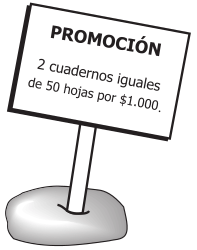
\includegraphics[scale=.45]{Images/Pantallazo-17.png} 
\end{center}}
\question \label{q01}
Con \$8.000, ¿cuántos cuadernos de la promoción se puede comprar sin que sobre dinero?

\begin{oneparchoices}
\choice 4
\choice 8
\choice 12
\CorrectChoice 16
\end{oneparchoices}
\question \label{q02}
¿En cuál de las siguientes tablas se muestra el precio correcto de 2, 4, 6 y 8 cuadernos iguales de 50 hojas?

\begin{choices}
\choice \begin{tabular}{|c|c|}
\hline 
\# cuadernos & Precio (\$) \\ 
\hline 
2 & 1000 \\ 
\hline 
4 & 2000 \\ 
\hline 
6 & 4000 \\ 
\hline 
8 & 8000 \\ 
\hline 
\end{tabular}
\choice \begin{tabular}{|c|c|}
\hline 
\# cuadernos & Precio (\$) \\ 
\hline 
2 & 500 \\ 
\hline 
4 & 1000 \\ 
\hline 
6 & 1500 \\ 
\hline 
8 & 2000 \\ 
\hline 
\end{tabular} 
\choice \begin{tabular}{|c|c|}
\hline 
\# cuadernos & Precio (\$) \\ 
\hline 
2 & 500 \\ 
\hline 
4 & 1000 \\ 
\hline 
6 & 2000 \\ 
\hline 
8 & 3000 \\ 
\hline 
\end{tabular} 
\CorrectChoice \begin{tabular}{|c|c|}
\hline 
\# cuadernos & Precio (\$) \\ 
\hline 
2 & 1000 \\ 
\hline 
4 & 2000 \\ 
\hline 
6 & 3000 \\ 
\hline 
8 & 4000 \\ 
\hline 
\end{tabular} 
\end{choices}
\question Pedro tenía algunos dulces guardados, se comió la mitad y regaló 2. Ahora tiene 4 dulces. ¿Cuántos dulces tenía guardados Pedro?

\begin{oneparchoices}
\choice 6
\choice 8
\choice 10
\CorrectChoice 12
\end{oneparchoices}
\question Para elaborar una tarjeta de felicitación, Marta dobló una hoja de papel por la mitad, como se indica a continuación:
\begin{center}
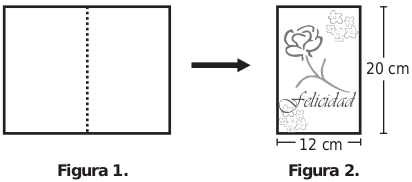
\includegraphics[scale=.45]{Images/Pantallazo-19.png} 
\end{center}
La tarjeta tiene las medidas indicadas en la figura 2.
¿Cuáles son las medidas de los lados de la hoja que Marta dobló?
\begin{choices}
\choice 10 y 6 cm
\CorrectChoice 20 y 24 cm
\choice 20 y 6 cm
\choice 10 y 12 cm
\end{choices}
\question El valor de la expresión 
$14-(2+5)+(-2)=$ es:
\begin{oneparchoices}
\choice $-5$
\choice $-9$
\CorrectChoice $5$
\choice $9$
\end{oneparchoices}
\question ¿Cuál de las siguientes frases NO se relaciona con el número $-32$?
\begin{choices}
\choice Ese matemático nació el año 32 antes de Cristo.
\choice La temperatura es 32$^{\circ}$C. bajo cero
\CorrectChoice El termómetro marca 32$^{\circ}$C
\choice Un submarino está 32 metros bajo el nivel del mar.
\end{choices}
\question La suma de dos enteros que tienen signos negativos es:
\begin{choices}
\choice No se puede determinar
\CorrectChoice Siempre un número negativo
\choice Siempre cero
\choice Siempre un número positivo
\end{choices}
\question  El resultado de $20+(-60)-40- 20$ es:

\begin{oneparchoices}
\choice 100
\CorrectChoice $-100$
\choice 140
\choice $-140$
\end{oneparchoices}
\question Calcula el valor de $3 - ((-7 + 4) + (8 - 3) - 5) =$

\begin{oneparchoices}
\choice 14
\choice $-14$
\CorrectChoice 6
\choice $-6$
\end{oneparchoices}
\question Después de subir 6 pisos el ascensor de un edificio llega al piso 5 ¿De qué planta ha salido?

\begin{oneparchoices}
\choice 6
\CorrectChoice $-1$
\choice 1
\choice 5
\end{oneparchoices}
\question La suma de dos números enteros que tienen signos diferentes es:
\begin{choices}
\choice  Siempre cero.
\choice Siempre un número entero negativo.
\CorrectChoice Depende del valor absoluto de los números.
\choice Siempre un número entero positivo.
\end{choices}
\question El número que corresponde a $x$ para que la igualda $40 + x = -5$ \quad sea verdadera es:

\begin{oneparchoices}
\choice 45
\choice 35
\choice $-35$
\CorrectChoice $-45$
\end{oneparchoices}
\question Un submarino de la flota naval, desciende a 50 metros bajo el nivel del mar y luego asciende a 20 metros. Entonces queda a una profundidad de:
\begin{choices}
\choice 30 metros sobre el nivel del mar
\CorrectChoice 30 metros bajo el nivel del mar
\choice 70 metros sobre el nivel del mar
\choice 70 metros bajo el nivel del mar
\end{choices}
%Pregunta
%\begin{oneparchoices}
%\choice[1] Nunca
%\end{oneparchoices}
%\answerline
\question
Número que al sustraerle (restarle) 549 da como resultado 8361:

\begin{oneparchoices}
\CorrectChoice 8910
\choice 9314
\choice 527
\choice 8361
\end{oneparchoices}
\question 
En un colegio hay 1000 estudiantes, en primaria hay 315 y en secundaria 187 más que en primaria. ¿Cuántos estudiantes hay en preescolar?

\begin{oneparchoices}
\choice 315
\CorrectChoice 183
\choice 190
\choice 685
\end{oneparchoices}
%cuadro de puntajes
%\begin{center}
%\gradetable[h][pages]
%\end{center}
\end{questions}
\end{multicols}
\end{document}